\documentclass[twocolumn, 10pt]{article}
\setlength\textwidth{6.875in}
\setlength\textheight{8.875in}
% set both margins to 2.5 pc
\setlength{\oddsidemargin}{-0.1875in}% 1 - (8.5 - 6.875)/2
\setlength{\evensidemargin}{-0.1875in}
\setlength{\marginparwidth}{0pc}
\setlength{\marginparsep}{0pc}%
\setlength{\topmargin}{0in} \setlength{\headheight}{0pt}
\setlength{\headsep}{0pt}
\setlength{\footskip}{37pt}%
%\setlength{\columnsep}{0.3125in}
%\setlength{\columnwidth}{3.28125in}% (6.875 - 0.3125)/2 = 3.28125in
\setlength{\parindent}{1pc}
\newcommand{\myMargin}{1.00in}
\usepackage[top=\myMargin, left=\myMargin, right=\myMargin, bottom=\myMargin, nohead]{geometry}
\usepackage{epsfig,graphicx}
\usepackage{palatino}
\usepackage{fancybox}
\usepackage{hyperref}
\usepackage[procnames]{listings}

% "define" Stanza
\usepackage[T1]{fontenc}  
\usepackage[scaled=0.82]{beramono}  
\usepackage{microtype} 

\sbox0{\small\ttfamily A}
\edef\mybasewidth{\the\wd0 }

\lstdefinelanguage{stanza}{
  morekeywords={circuit, defclass,defmodule,defbundle,definterface,defpackage,defn,%
    do,else,public,false,finally,%
    for,if,import,inherit,inst,match,%
    map,new,node,object,override,package,%
    super,this,throw,true,try,%
    type,val,var,when,while%,
    % yield,UInt,Bool,Bits,SInt
    },
  sensitive=true,
  morecomment=[l]{;;},
  morestring=[b]",
  morestring=[b]',
  morestring=[b]"""
}

\usepackage{color}
\definecolor{dkgreen}{rgb}{0,0.6,0}
\definecolor{gray}{rgb}{0.5,0.5,0.5}
\definecolor{mauve}{rgb}{0.58,0,0.82}

% Default settings for code listings
\lstset{frame=tb,
  language=stanza,
  aboveskip=3mm,
  belowskip=3mm,
  showstringspaces=false,
  columns=fixed, % basewidth=\mybasewidth,
  basicstyle={\small\ttfamily},
  numbers=none,
  numberstyle=\footnotesize\color{gray},
  % identifierstyle=\color{red},
  keywordstyle=\color{blue},
  commentstyle=\color{dkgreen},
  stringstyle=\color{mauve},
  frame=single,
  breaklines=true,
  breakatwhitespace=true,
  procnamekeys={input,output,wire, mem, reg, node, defn, val, var, defclass, definterface, defbundle, defmodule, defpackage},
  procnamestyle=\ttfamily\color{red},
  tabsize=2
}

\lstnewenvironment{stanza}[1][]
{\lstset{language=stanza,#1}}
{}

% "define" Stanza
\usepackage[T1]{fontenc}  
\usepackage[scaled=0.82]{beramono}  
\usepackage{microtype} 

\sbox0{\small\ttfamily A}
\edef\mybasewidth{\the\wd0 }

\lstdefinelanguage{stanza}{
  morekeywords={circuit, defclass,defmodule,defbundle,definterface,defpackage,defn,%
    do,else,public,false,finally,%
    for,if,import,inherit,input,inst,match,%
    map,mem,new,node,object,override,output,package,%
    reg,super,this,throw,true,try,%
    type,val,var,when,while,wire%,%
    % yield,UInt,Bool,Bits,SInt
    },
  sensitive=true,
  morecomment=[l]{;;},
  morestring=[b]",
  morestring=[b]',
  morestring=[b]"""
}

\usepackage{color}
\definecolor{dkgreen}{rgb}{0,0.6,0}
\definecolor{gray}{rgb}{0.5,0.5,0.5}
\definecolor{mauve}{rgb}{0.58,0,0.82}

% Default settings for code listings
\lstset{frame=tb,
  language=stanza,
  aboveskip=3mm,
  belowskip=3mm,
  showstringspaces=false,
  columns=fixed, % basewidth=\mybasewidth,
  basicstyle={\small\ttfamily},
  numbers=none,
  numberstyle=\footnotesize\color{gray},
  % identifierstyle=\color{red},
  keywordstyle=\color{blue},
  commentstyle=\color{dkgreen},
  stringstyle=\color{mauve},
  frame=single,
  breaklines=true,
  breakatwhitespace=true,
  procnamekeys={input,output,wire, mem, reg, node, defn, val, var, defclass, definterface, defbundle, defmodule, defpackage},
  procnamestyle=\ttfamily\color{red},
  tabsize=2
}




\lstset{basicstyle={\footnotesize\ttfamily}}

\newenvironment{commentary}
{ \vspace{-0.1in}
  \begin{quotation}
  \noindent
  \small \em
  \rule{\linewidth}{1pt}\\
}
{
  \end{quotation}
}

\title{Getting Started: Tutorial 01 - The Basics}
\author{Jonathan Bachrach, Vincent Lee \\
EECS Department, UC Berkeley\\
{\tt  \{jrb\}@eecs.berkeley.edu}
}
\date{\today}

\newenvironment{example}{\VerbatimEnvironment\begin{footnotesize}\begin{Verbatim}}{\end{Verbatim}\end{footnotesize}}
\newcommand{\kode}[1]{\begin{footnotesize}{\tt #1}\end{footnotesize}}

\def\code#1{{\tt #1}}

\def\note#1{\noindent{\bf [Note: #1]}}
%\def\note#1{}

\begin{document}
\maketitle{}

\subsection{The Chisel Directory Structure}

Once you have acquired the tutorial files you should see the following Chipper tutorial directory structure under \verb+$TUT_DIR+:

\begin{bash}
chipper-tutorial/  
  Makefile
  examples/   # chipper examples
    Makefile  # for running examples
    Accumulator.stanza ...
  problems/   # skeletal files for tutorial problems
    Makefile  # for running / testing problems
    Counter.stanza ...
  solutions/  # solutions to problems
    Makefile  # for running solutions
    Counter.stanza ...
\end{bash}

Chipper source files are distributed between \verb+examples+, \verb+problems+, and \verb+solutions+ directories.
The tutorial contains the files that you will be modifying under \verb+problems/+ while the \verb+solutions/+ folder contains the reference implementations for each of the problems.  Finally, \verb+examples/+ contains source to the complete examples given in this tutorial.

Finally, the \verb+build.sbt+ files contain the build configuration information used to specify what version of Chipper to make your project with.

\section{Running Your First Chipper Build}

In this section, we explain how to run your first build to explore what Chipper has to offer. We will go through a simple example for a GCD module and familiarize ourselves with the source files, simulation, and Verilog generation. More comprehensive details will follow in subsequent sections of the tutorial.

\subsection{The Chipper Source Code}

Now that you are more familiar with what your Chipper directory structure contains, let's start by exploring one of the Chipper files. Change directory into the \verb+examples/+ directory and open up the \verb+GCD.stanza+ file with your favorite text editor. 

You will notice that file is already filled out for you to perform the well known GCD algorithm and should look like:

\begin{stanza}
#use-syntax(core, chipper)

defpackage GCD :
   import core
   import verse
   import chipper

defmodule GCD :
   input a: UInt<16>
   input b: UInt<16>
   input e: UInt<1>
   output z: UInt<16>
   output v: UInt<1>

   reg x: UInt<16>
   reg y: UInt<16>
   when x > y :
      x := x - y
   else :
      y := y - x
   when e :
      x := a
      y := b
   z := x
   v := y === UInt(0)
\end{stanza}

The first thing you will notice is the \verb+import Chipper+ declaration; this imports the Chipper library files that allow us to leverage Stanza as a hardware construction language. After the import declarations you will see the Chipper module definition for the Chipper component you are implementing. You can think of this as almost the same thing as a module declaration in Verilog.

Next we see the I/O specification for this component in the \verb+input+ and \verb+output+ definitions. You will notice that there is a line for each port specifying the direction (either \verb+input+ or \verb+output+), name, and type (e.g., \verb+UInt+, \verb+Bool+, etc.). If a bit width is not specified, Chipper will infer the appropriate bit width for you (in this case default to 1). 

The next section of code performs the actual GCD computation for the module. The register declarations for \verb+x+ and \verb+y+ tell Chipper to treat \verb+x+ and \verb+y+ as a register of type UInt(). 

\begin{stanza}
reg x : UInt<16> // declares x as UInt register
reg y : UInt<16> // declares y as UInt register
\end{stanza}

The \verb+when+ statement tells Chipper to perform the operation on a positive clock edge if the condition is true, treating the left hand assignments as synchronous. This is similar to how Verilog uses \verb+always @ (posedge clk)+ to specify synchronous logic.

Finally we see the output assignments for the computation for \verb+z+ and \verb+v+. One particular thing to notice is that, we do not have to specify the width of \verb+x+ and \verb+y+ in this example. This is because Chipper does the bit width inference for you and sets these values to their appropriate widths based on the computation they are storing.

\subsection{Running the Chipper Simulation}

Now that we are familiar with the Chipper code for the \verb+GCD.stanza+ file, let's try to simulate it by generating the simulation models. Change directory into the \verb+$DIR/examples/+ directory. Here you will see one lonely Makefile which we will call with:

\begin{bash}
make GCD.out
\end{bash}

\noindent
This will fire off the Chipper emulator that will run the simulation for the component defined in \verb+GCD.stanza+. If the simulation succeeds, you should see some debug output followed by:
\begin{footnotesize}
\begin{bash}
PASSED
[success] Total time: 2 s, completed Feb 28, 2013 \
  8:14:37 PM
\end{bash}
\end{footnotesize}

The debug output is generated by the test harness which composes the second half of the GCD.stanza file. We will talk about this more later. In addition to the debug output, the build also creates simulation models which can be used to simulate and debug more complicated designs.

\subsection{Generating the Verilog}

One of the most powerful features of Chipper is its ability to generate FPGA and ASIC Verilog from the Stanza sources that you construct. To do this, change directory into the \verb+$DIR/examples/verilog/+ directory and again run:
\begin{bash}
make GCD.v
\end{bash}
This will start the Verilog generation for the GCD Chipper file. When the Verilog generation finishes, you should see a [success] message similar to the one you saw in the emulator and a new \verb+GCD.v+ file. If you open up \verb+GCD.v+, you will find that Chipper has compiled \verb+GCD.stanza+ into its equivalent Verilog source.

You will find that the Chipper compiler has generated an equivalent Verilog module that performs the GCD computation.

The Verilog source is roughly divided into three parts:
\begin{enumerate}
\item Module declaration with input and outputs
\item Temporary wire and register declaration used for holding intermediate values
\item Register assignments in \verb+always @ (posedge clk)+
\end{enumerate}

\section{Combinational Logic}

\subsection{Declaring Wires}

Constructing combinational logic blocks in Chipper is fairly straightforward; when you declare a \verb+node+ in Stanza, it creates a node that represents the data that it is assigned to. As long as the value is not assigned to be a register type (explained later), this tells the Chipper compiler to treat the value as wire. Thus any number of these values can be connected and manipulated to produce the value that we want.

Suppose we want to construct a single full adder. A full adder takes two inputs \verb+a+ and \verb+b+, and a carry in \verb+cin+ and produces a \verb+sum+ and carry out \verb+cout+. The Chipper source code for our full adder will look something like:

\begin{stanza}
defmodule FullAdder :
   input a:     UInt<1>
   input b:     UInt<1>
   input cin:   UInt<1>
   output sum:  UInt<1>
   output cout: UInt<1>

  ;; Generate the sum
  wire a_xor_b = a ^ b
  ;; Reassignment to sum so use :=
  sum := a_xor_b ^ cin 
  // Generate the carry
  wire a_and_b = a & b
  wire b_and_cin = b & cin
  wire a_and_cin = a & cin
  ;; reassignment to cout so use :=
  cout := a_and_b | b_and_cin | a_and_cin
\end{stanza}

\noindent
where \verb+cout+ is defined as a combinational function of inputs \verb+a+, \verb+b+, and \verb+cin+.  The |, \&, and \^\ operators correspond to bitwise OR, AND, and XOR operations respectively.

The corresponding wires for each of these values is shown below in Figure~\ref{fig:full-adder}.  You will notice that each \verb+wire+ corresponds to exactly one of the wires.

\begin{figure}[ht!]
\centering
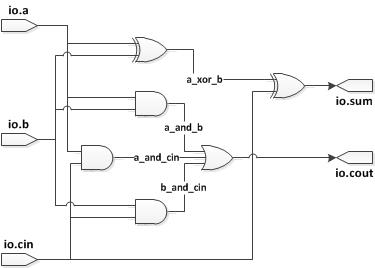
\includegraphics[width=80mm]{figs/Full_Adder.jpg}
\caption{Full Adder Circuit}
\label{fig:full-adder}
\end{figure}


\subsection{Bit Width Inference}

If you don't explicitly specify the width of a value in Chipper, the Chipper compiler will infer the bit width for you based on the inputs that define the value. Notice in the \verb+FullAdder+ definition, the widths for \verb+a_xor_b, a_and_b, b_and_cin,+ and \verb+a_and_cin+ are never specified anywhere. However, based on how the input is computed, Chipper will correctly infer each of these values are one bit wide since each of their inputs are the results of bitwise operations applied to one bit operands.

A quick inspection of the generated Verilog shows these values are indeed one bit wide:

\begin{bash}
module FullAdder(
    input  a,
    input  b,
    input  cin,
    output sum,
    output cout);

  wire T0;
  wire a_and_cin;
  wire T1;
  wire b_and_cin;
  wire a_and_b;
  wire T2;
  wire a_xor_b;

  assign cout = T0;
  assign T0 = T1 | a_and_cin;
  assign a_and_cin = a & cin;
  assign T1 = a_and_b | b_and_cin;
  assign b_and_cin = b & cin;
  assign a_and_b = a & b;
  assign sum = T2;
  assign T2 = a_xor_b ^ cin;
  assign a_xor_b = a ^ b;
endmodule
\end{bash}

Suppose we change the widths of the \verb+FullAdder+ to be 2 bits wide each instead such that the Chipper source now looks like:

\begin{stanza}
defmodule FullAdder :
  input a:     UInt<2>
  input b:     UInt<2>
  input cin:   UInt<2>
  output sum:  UInt<2>
  output cout: UInt<2>

  ;; Generate the sum
  wire a_xor_b = a ^ b
  ;; Reassignment to sum so use :=
  sum := a_xor_b ^ cin 
  // Generate the carry
  wire a_and_b = a & b
  wire b_and_cin = b & cin
  wire a_and_cin = a & cin
  ;; reassignment to cout so use :=
  cout := a_and_b | b_and_cin | a_and_cin
\end{stanza}

As a result, the Chipper compiler should infer each of the intermediate values \verb+a_xor_b, a_and_b, b_and_cin,+ and \verb+a_and_cin+ are two bits wide. An inspection of the Verilog code correctly shows that Chipper inferred each of the intermediate wires in the calculation to be 2 bits wide.

\begin{bash}
module FullAdder(
    input [1:0] a,
    input [1:0] b,
    input [1:0] cin,
    output[1:0] sum,
    output[1:0] cout);

  wire[1:0] T0;
  wire[1:0] a_and_cin;
  wire[1:0] T1;
  wire[1:0] b_and_cin;
  wire[1:0] a_and_b;
  wire[1:0] T2;
  wire[1:0] a_xor_b;

  assign cout = T0;
  assign T0 = T1 | a_and_cin;
  assign a_and_cin = a & cin;
  assign T1 = a_and_b | b_and_cin;
  assign b_and_cin = b & cin;
  assign a_and_b = a & b;
  assign sum = T2;
  assign T2 = a_xor_b ^ cin;
  assign a_xor_b = a ^ b;
endmodule
\end{bash}

\section{Using Registers}

Unlike Verilog, specifying a register in Chipper tells the compiler to actually generate a positive edge triggered register. In this section we explore how to instantiate registers in Chipper by constructing a shift register.

In Chipper, when you instantiate a register there are several ways to specify the connection of the input to a register. As shown in the GCD example, you can ``declare'' the register and assign what it's input is connected to in a \verb+when...+ block or you can simply assign the value that the register is clocking.

If you choose to specify the a next value at register construction, it will clock the new value every cycle unconditionally:

\begin{stanza}
;; Clock the new register value on every cycle
wire y = x + x
reg z := y
\end{stanza}

If we only want to update if certain conditions are met we use a \verb+when+ block to indicate that the registers are only updated when the condition is satisfied:

\begin{stanza}
// Clock the new register value when the condition a > b
reg x : UInt
when a > b :      x := y
else: when b > a: x := z
else:             x := w
\end{stanza}

It is important to note that when using the conditional method, the values getting assigned to the input of the register match the type and bitwidth of the register you declared. In the unconditional register assignment, you do not need to do this as Chipper will infer the type and width from the type and width of the input value.

The following sections show how these can be used to construct a shift register.

\subsection{Unconditional Register Update}

Suppose we want to construct a basic 4 bit shift register that takes a serial input \verb+in+ and generates a serial output \verb+out+. For this first example we won't worry about a parallel load signal and will assume the shift register is always enabled. We also will forget about the register reset signal.

If we instantiate and connect each of these 4 registers explicitly, our Chipper code will look something like:

\begin{stanza}
defmodule ShiftRegister :
  input  in:  UInt<1>
  output out: UInt<1>

  reg r0 := in
  reg r1 := r0
  reg r2 := r1
  reg r3 := r2

  out := r3
\end{stanza}

If we take a look at the generated Verilog, we will see that Chipper did indeed map our design to a shift register. One thing to notice is that the clock signal and reset signals are implicitly attached to our design.

\begin{bash}
module ShiftRegister(input clk, input reset,
    input  in,
    output out);

  reg[0:0] r3;
  reg[0:0] r2;
  reg[0:0] r1;
  reg[0:0] r0;

  assign out = r3;
  always @(posedge clk) begin
    r3 <= r2;
    r2 <= r1;
    r1 <= r0;
    r0 <= in;
  end
endmodule
\end{bash}

\subsection{Conditional Register Update}

As mentioned earlier, Chipper allows you to conditionally update a register (use an enable signal) using the \verb+when+, \verb+else when+, \verb+else+ block. Suppose we add an enable signal to our shift register, that allows us to control whether data is shift in and out on a given cycle depending on an \verb+enable+ input signal. The new shift register now looks like:

\begin{stanza}
defmodule ShiftRegister :
  input  in:     UInt<1>
  input  enable: Bool
  output out:    UInt<1>

  reg r0 : UInt
  reg r1 : UInt
  reg r2 : UInt
  reg r3 : UInt

  when enable :
    r0 := in
    r1 := r0
    r2 := r1
    r3 := r2

  out := r3
\end{stanza}

Notice that it is not necessary to specify an \verb+else+ condition as Chipper will correctly infer that the old register value should be preserved otherwise.

\subsection{Register Reset}

Chipper allows you to specify a synchronous reset to a certain value by specifying an additional parameter when you first declare them. In our shift register, let's add a reset capability that resets all the register values to zero synchronously. To do this we need to provide our register declarations a little more information using the \verb+=+ syntax specifying what value we want on a synchronous reset:

\begin{stanza}
defmodule ShiftRegister :
  input  in:     UInt<1>
  input  enable: Bool
  output out:    UInt<1>

  reg r0 = UInt(0)
  reg r1 = UInt(0)
  reg r2 = UInt(0)
  reg r3 = UInt(0)

  when enable :
    r0 := in
    r1 := r0
    r2 := r1
    r3 := r2

  out := r3
\end{stanza}

Notice that reset value can actually be any value, simply replace the zeros and width to appropriate values.

Chipper also has an implict global \verb+reset+ signal that you can use in a \verb+on-reset+ statement. The shift register using this implict global reset now looks like:

\begin{stanza}
defmodule ShiftRegister :
  input  in:     UInt<1>
  input  enable: Bool
  output out:    UInt<1>

  reg r0 : UInt
  reg r1 : UInt
  reg r2 : UInt
  reg r3 : UInt

  on-reset : r0 := UInt(0)
  on-reset : r1 := UInt(0)
  on-reset : r2 := UInt(0)
  on-reset : r3 := UInt(0)

  when enable :
    r0 := in
    r1 := r0
    r2 := r1
    r3 := r2

  out := r3
\end{stanza}

This will generate slightly different looking Verilog source code but will still function the same as the previous implementation of the shift register with reset.

% HOW TO DO THIS FOR YOUR OWN RESET SIGNALS

\subsection{\problem{Sequential Circuit}}

The following exercises can be found in your \verb+$TUT_DIR/problems/+ folder. You will find that some parts of the tutorial files have been completed for you and the section that you need to will need to complete is indicated in the file. The solutions to each of these exercises can be found in the \verb+$TUT_DIR/solutions/+ folder.

The first tutorial problem is to write write a sequential circuit that sums \verb+in+ values. 
You can find the template in \verb+$TUT_DIR/problems/Accumulator.stanza+ including a stubbed out version of the circuit:
\begin{stanza}
defmodule Accumulator :
  input  in  : UInt<1>
  output out : UInt<8>

  ;; flush this out ...

  out := UInt(0)
\end{stanza}

\noindent
and a complete tester that confirms that you have successfully designed the circuit.  Run 

\begin{bash}
make Accumulator.out
\end{bash}

\noindent 
until your circuit passes the tests.


%\subsection{Creating a Two Input Multiplexor}
%
%<IS THIS EVEN A GOOD IDEA BECAUSE THEY DON'T REALLY KNOW ANYTHING YET>
%
%\subsection{Creating a Simple FIFO}
%
%<IS THIS EVEN A GOOD IDEA BECAUSE THEY DON'T REALLY KNOW ANYTHING YET>
%


\end{document}
